\chapter{PyMUVs}

{
\color{red}
PyMUVs-kapitellet kan godt utvides en god del. Sensor vet ingenting om hvor mye tid du har brukt på debugging og implementering, så det må komme fram at dette er noe du har brukt mye tid på og som er en viktig del av bidraget ditt.
\begin{itemize}
    \item Should this be a chapter?
    \item how relevant is this?
    \item Nevn Gazebo, og at man ikke kan hente ut modellmatriser derifra, så det ikke er en fullstendig løsning for modellbasert styring av roboter.
    \item Forklar hvordan det er implementert, med matematikken bak. Stor forskjell i en prosjektoppgave på å sitere modsimboka og på å implementere en dynamisk simulator fra scratch.
    \item Beskriv hvordan systmet er definert i koden din
\end{itemize}
}

\emph{\textbf{Py}MUVs \textbf{M}odels \textbf{U}nderwater \textbf{V}ehicle\textbf{s}}
\newline

PyMUVs is a Python library for mathematically modelling underwater vehicles. The
library is designed to be modular and easy to use, and is built on top of NumPy
\cite{numpy} and SymPy \cite{sympy}. By defining the a set of links and transformations
between them, \pymuvs can compute a symbolic representation of the system on the
form
\begin{align}
    \bm{M}(\bm{q}) \ddot{\bm{q}} + \bm{C}(\bm{q}, \dot{\bm{q}}) \dot{\bm{q}} +
    \bm{D}(\bm{q}, \dot{\bm{q}}) \dot{\bm{q}} + \bm{g}(\bm{q}) = \bm{J}^T(\bm{q}) \bm{B} \bm{u}
    \label{eq:pymuvs:eom}
\end{align}
The matrices $\bm{M}$, $\bm{C}$, $\bm{D}$, $\bm{g}$, $\bm{J}$, and $\bm{B}$ are
computed symbolically and can be used to simulate the system. This is especially
usefull when implementing model-based controllers that require the dynamics of the
system to be on the form of, or similar to \autoref{eq:pymuvs:eom}. The library
also supports exporting the symbolic representation, and the whole model to C++
code, which can be used in real-time simulations or for significantly faster
simulations. The library being written in python allows for quick and easy
prototyping of models, being able to remove and add links and transformations.
The library is open-source and can be found at
\url{https://github.com/haakonbaa/pymuvs}. 

\section{Modules}
The following sections will give an overview of the modules making up the
library as well as some breif examples showing basic use cases. Note that this
is not a complete overview of the library, but rather a brief introduction to
the most important functionality of each module.

% ------------------------------------------------------------------------- se3
\subsection{se3}
The \texttt{se3} module contains functions for working with the special Euclidean
group $SE(3)$. The module is built on top of \texttt{SymPy} and provides functions for
generating elements of $SE(3)$ from \texttt{SymPy} symbols, as well as functions
for computing the inverse and multiplication of the elements. A simple example
is shown below.

\begin{figure}[h]
    \centering
    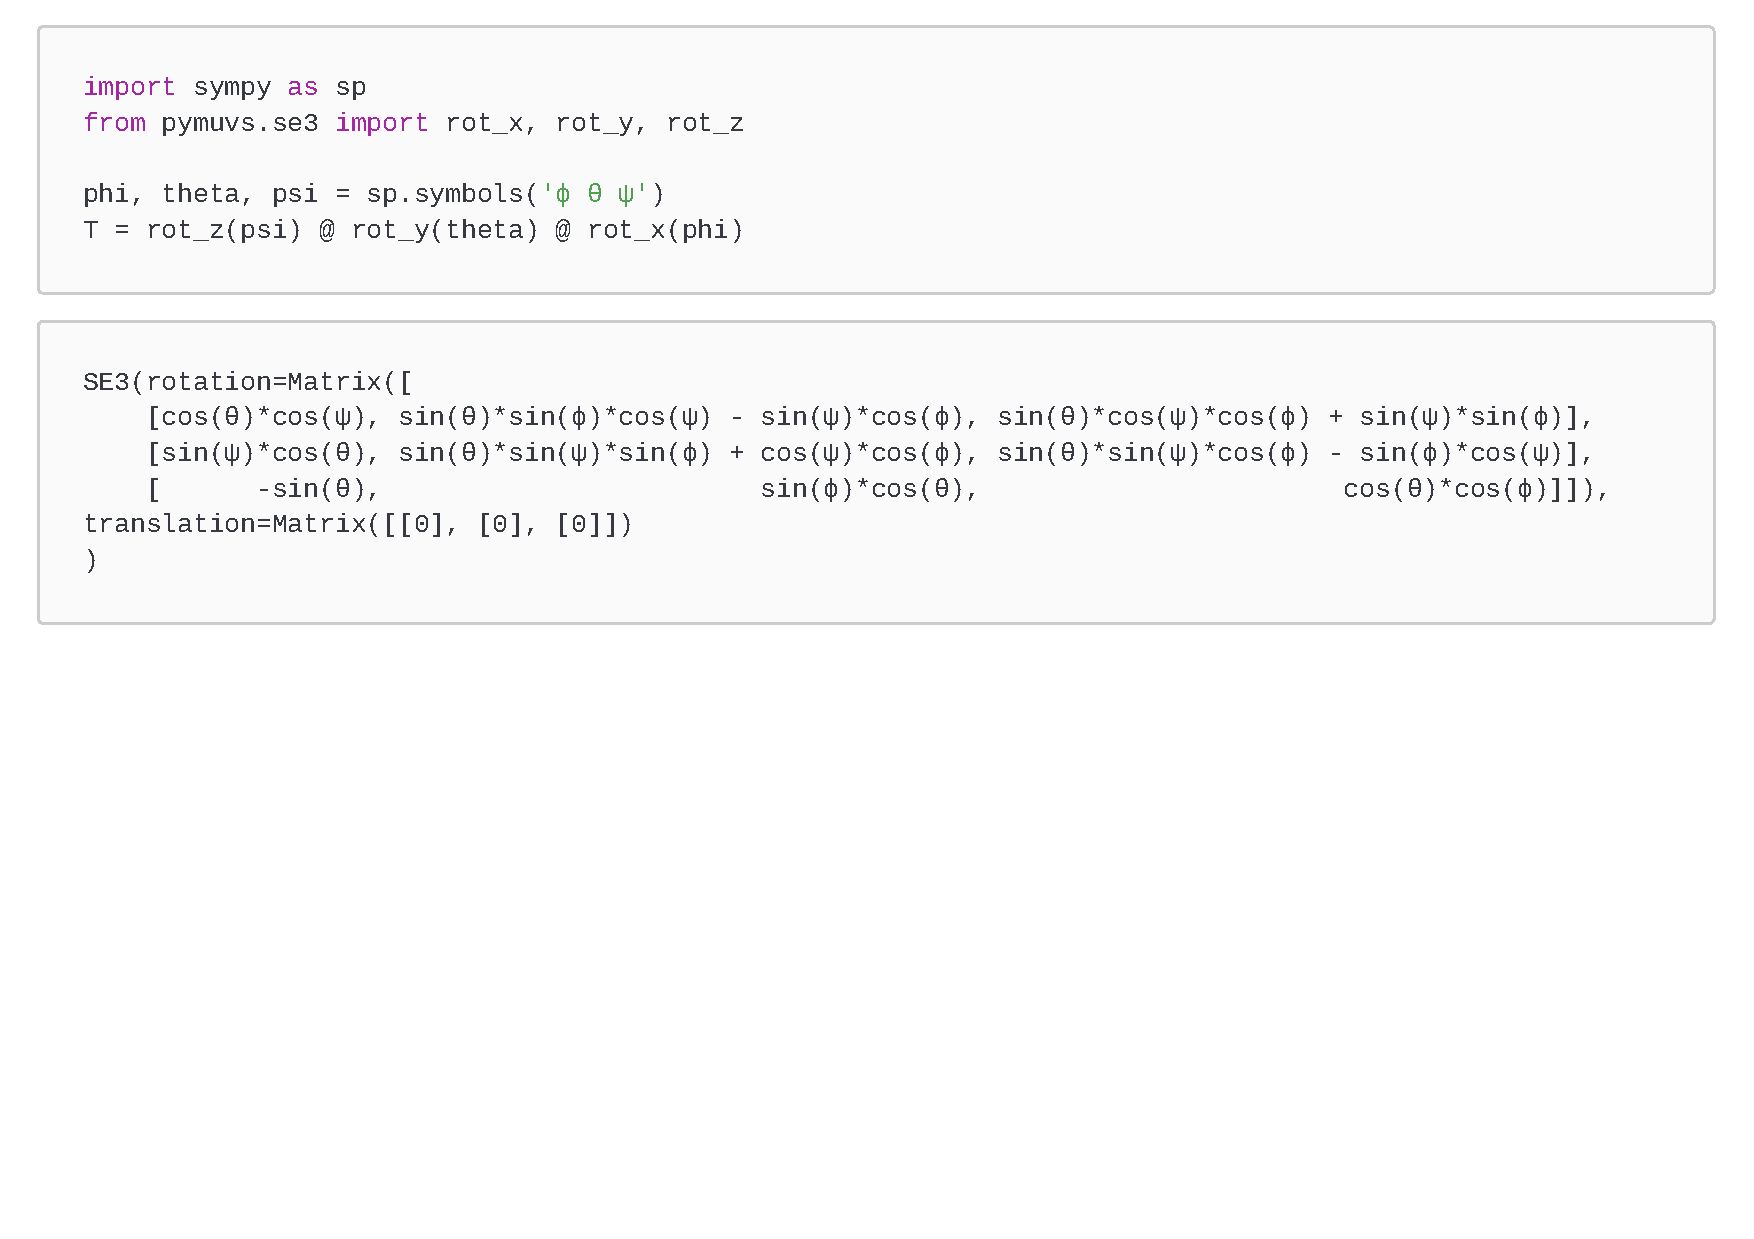
\includegraphics[page=1,width=\linewidth,trim=0 11cm 0 0]{assets/se3.pdf}
    \caption{Example usage of the \texttt{se3} module.}
    \label{fig:usage:se3}
\end{figure}

\autoref{fig:usage:se3} shows how to create a variable $T \in \SO$ representing
a pure rotation in euler angles. More elements of this calss can be composed
together to form arbitrary transformations. This group is used in other modules
to represent the transformations between links in a robot model.

% --------------------------------------------------------------------- util
\subsection{util}


% --------------------------------------------------------------------- codegen
\subsection{codegen}
The \texttt{codegen} module is used to generate C++ code from a model. The module
uses the \texttt{sympy.ccode} function to generate C code from
each expression in every matrix and combines them into a header and a source
file. The \texttt{Eigen} library \cite{eigen3} is used to represent the matrices.

\begin{figure}[h]
    \centering
    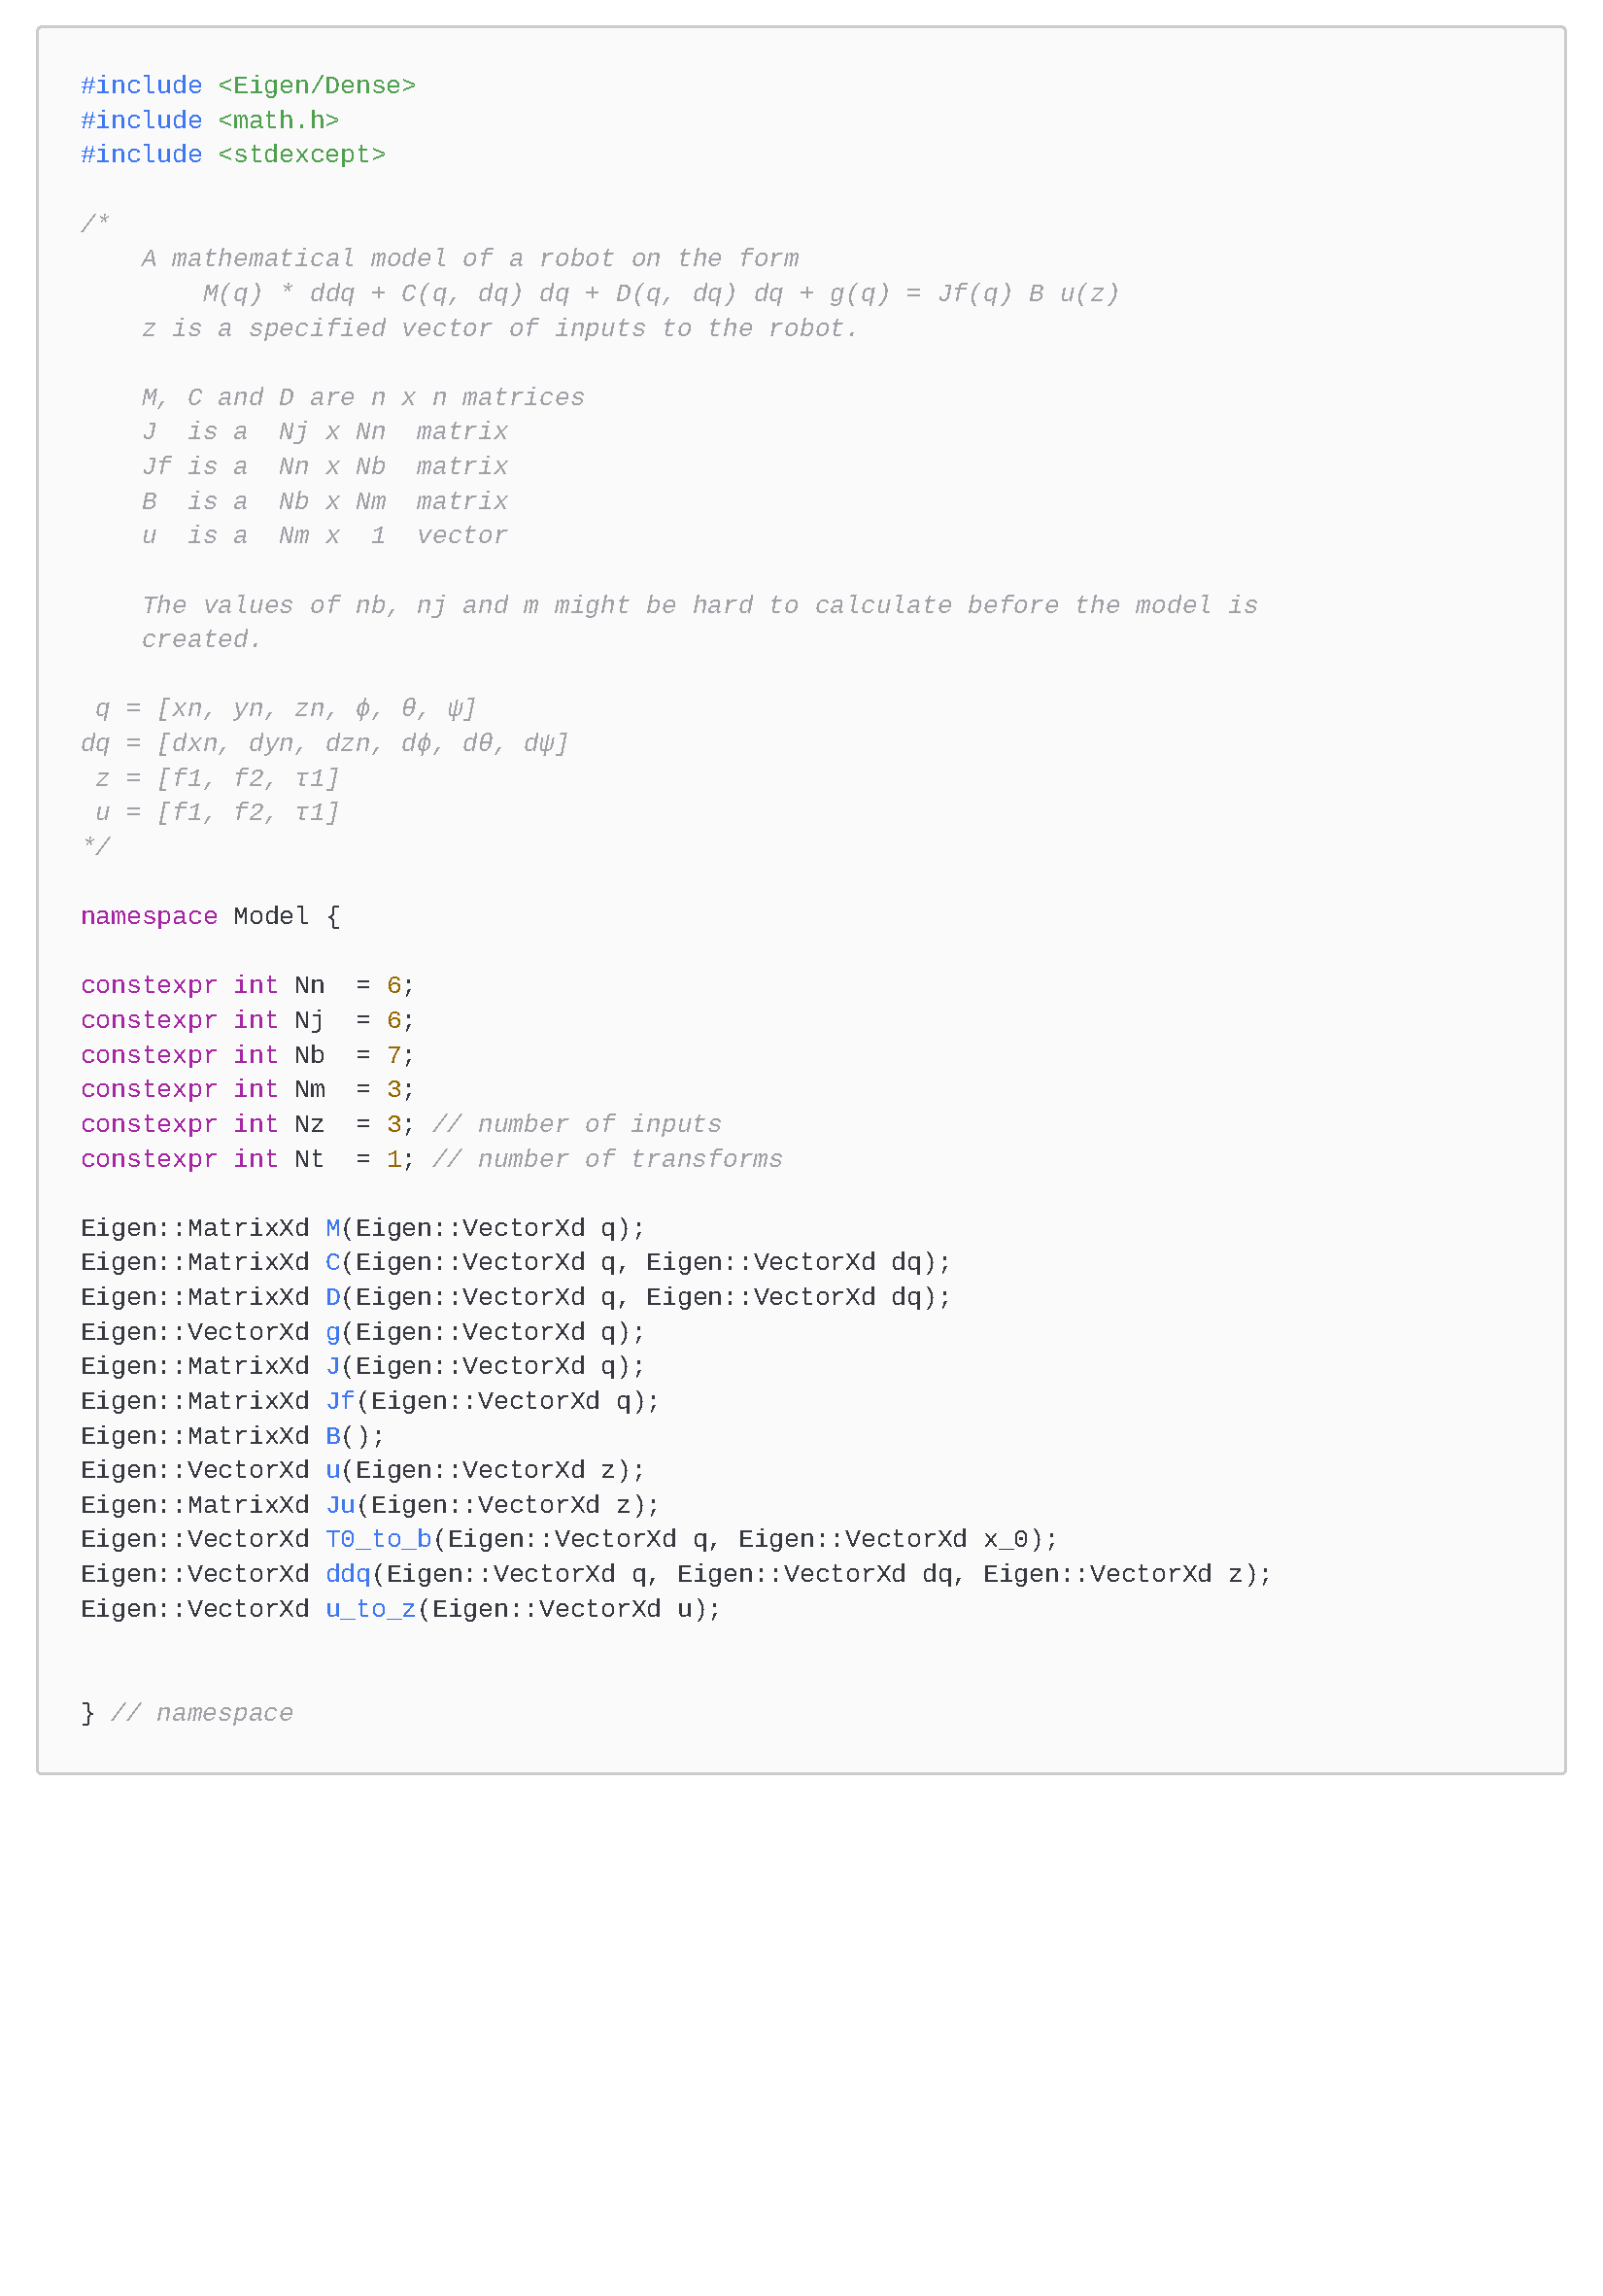
\includegraphics[page=1,width=\linewidth,trim=0 9cm 0 0]{assets/codegen.pdf}
    \caption{Automatically generated c++ code from a model.}
    \label{fig:codegen}
\end{figure}

\subsection{pymuvs}
